%%%%%%%%%%%%%%%%%%%%%%%%%%%%%%%%%%%%%%%%%%%%
%%%%%                                  %%%%%
%%%%%     DIMENSIONALITY REDUCTION     %%%%%
%%%%%                                  %%%%%     
%%%%%%%%%%%%%%%%%%%%%%%%%%%%%%%%%%%%%%%%%%%%     

\begin{frame}[t, c]{}{}
  \begin{minipage}{.48\textwidth}
    \centering
    {
      \Large\textbf{Part I}
    }
    
    \bigskip
    
    \rule{\textwidth}{0.001\textwidth}
    
    \bigskip
    
    {
      \large
      \textbf{Dimensionality reduction}
    }
    
    \medskip
    
    \begin{itemize}
    \item Problem formulation:
      \begin{itemize}
      \item[\(	\hookrightarrow \)] DMD as a Reduced Rank Regression
      \item[\( \hookrightarrow	\)] Linear autoencoder + linear dynamics
      \end{itemize}
      
      \medskip
      
    \item Practical usage:
      \begin{itemize}
      \item[\(	\hookrightarrow	\)] Extracting patterns from our flow
      \item[\(	\hookrightarrow \)] Low-dimensional embedding
      \end{itemize}
      
    \end{itemize}
    
  \end{minipage}%
  \hfill
  \begin{minipage}{.48\textwidth}
    \centering
    \movie[width=\textwidth, autostart, loop]{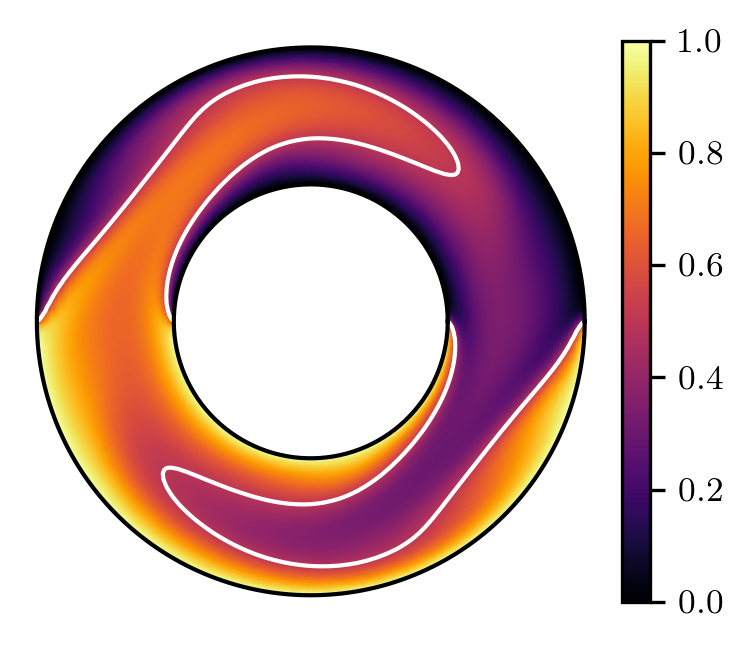
\includegraphics[width=\textwidth]{temperature_field_00000}}{imgs/temperature_evolution.mp4}
  \end{minipage}
\end{frame}

\begin{frame}[t, c]{Dynamic Mode Decomposition}{Problem formulation}
  \begin{minipage}{.68\textwidth}
    \begin{itemize}
    \item Given a discrete-time system \( \bm{x}_{k+1} = \bm{f}(\bm{x}_k) \), DMD aims to find a (low-rank) linear operator \( \bm{A} \) such that
      % 
      \[
        \begin{aligned}
          \minimize_{\bm{A}} & \sum_{k=1}^n \| \bm{f}(\bm{x}_k) - \bm{Ax}_k \|_2^2 \\
          \subjecto & \text{rank } \bm{A} = r.
        \end{aligned}
      \]
      
      \medskip
      
    \item This problem belongs to the class of \emph{Reduced-Rank Regression} problems.
    \end{itemize}
  \end{minipage}%
  \hfill
  \begin{minipage}{.28\textwidth}
    \centering
    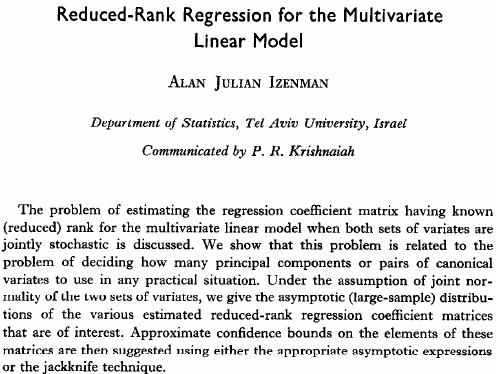
\includegraphics[width=\textwidth]{abstract_rrr}
  \end{minipage}
  
  \vspace{1cm}
\end{frame}

\begin{frame}[t, c]{Dynamic Mode Decomposition}{Matrix formulation and unconstrained solution}
  \begin{minipage}{.28\textwidth}
    \centering
    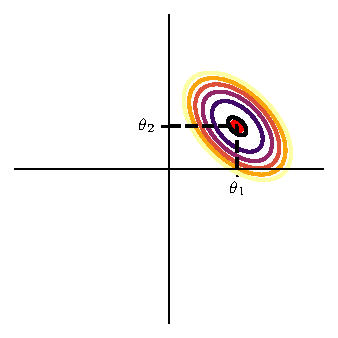
\includegraphics[width=\textwidth]{least_squares}
  \end{minipage}%
  \hfill
  \begin{minipage}{.68\textwidth}
    \begin{itemize}
    \item Problem can be recast in matrix form as
      % 
      \[
        \begin{aligned}
          \minimize_{\bm{A}} & \| \bm{Y} - \bm{AX} \|_F^2 \\
          \subjecto & \text{rank } \bm{A} = r,
        \end{aligned}
      \]
      % 
      where \( \bm{Y} = \bm{X}_{k+1} \) and \( \bm{X} = \bm{X}_k \).
      
      \medskip
      
    \item \underline{Unconstrained solution} is simply the least-squares solution
      % 
      \[
        \bm{A} = \bm{C}_{\bm{yx}} \bm{C}_{\bm{xx}}^{-1},
      \]
      % 
      with \( \bm{C}_{\bm{yx}} = \bm{YX}^H \) and \( \bm{C}_{\bm{xx}} = \bm{XX}^H \).
    \end{itemize}
  \end{minipage}
  
  \vspace{1cm}
\end{frame}

\begin{frame}[t, c]{Dynamic Mode Decomposition}{Rank-constrained solution}
  \begin{minipage}{.68\textwidth}
    \begin{itemize}
    \item Introducing the low-rank factorization \( \bm{A} = \bm{PQ}^H \), the minimization problem reads
      % 
      \[
        \begin{aligned}
          \minimize_{\bm{P}, \bm{Q}} & \| \bm{Y} - \bm{PQ}^H \bm{X} \|_F^2 \\
          \subjecto & \text{rank } \bm{P} = \text{rank } \bm{Q} = r \\
          & \bm{P}^H \bm{P} = \bm{I}.
        \end{aligned}
      \]
      
      \medskip
      
    \item \( \bm{P} \) is a basis for the column-span of \( \bm{A} \) while \( \bm{Q} \) is a basis for its row-span.
      These are in general different.
    \end{itemize}
  \end{minipage}%
  \hfill
  \begin{minipage}{.28\textwidth}
    \centering
    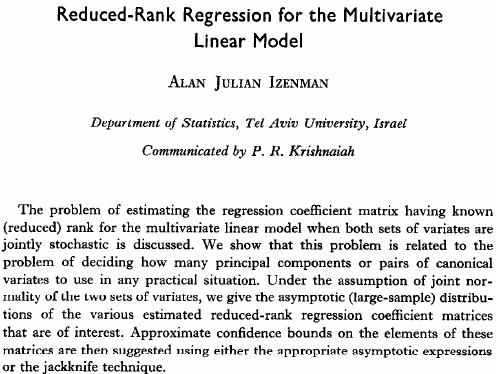
\includegraphics[width=\textwidth]{abstract_rrr}
  \end{minipage}
  
  \vspace{1cm}
\end{frame}

\begin{frame}[t, c]{Dynamic Mode Decomposition}{Rank-constrained solution}
  \begin{minipage}{.28\textwidth}
    \centering
    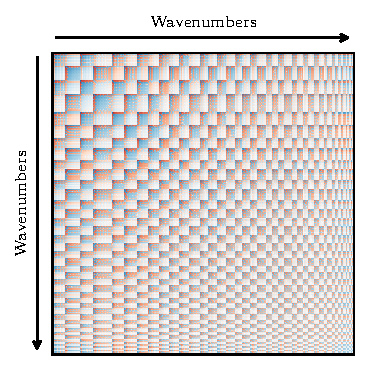
\includegraphics[width=\textwidth]{dmd_matrix}
  \end{minipage}%
  \hfill
  \begin{minipage}{.68\textwidth}
    \begin{itemize}
    \item Our minimization problem is equivalent to
      % 
      \[
        \begin{aligned}
          \maximize_{\bm{P}} & \text{Tr}\left( \bm{P}^H \bm{C}_{\bm{yx}} \bm{C}_{\bm{xx}}^{-1} \bm{C}_{\bm{xy}} \bm{P} \right) \\
          \subjecto & \text{rank } \bm{P} = r \\
          & \bm{P}^H \bm{P} = \bm{I}.
        \end{aligned}
      \]
      
      \medskip
      
    \item Optimal solution is given by the first \( r \) eigenvectors of the symmetric positive-definite matrix \( \bm{C}_{\bm{yx}} \bm{C}_{\bm{xx}}^{-1} \bm{C}_{\bm{xy}} \).
      
      \medskip
      
    \item \( \bm{Q} \) is solution to \( \bm{C}_{\bm{xx}} \bm{Q} =  \bm{C}_{\bm{xy}} \bm{P} \).
    \end{itemize}
  \end{minipage}
  
  \vspace{1cm}
\end{frame}

\begin{frame}[t, c]{Dynamic Mode Decomposition}{Dimensionality reduction and linear model}
  \begin{itemize}
  \item Once \( \bm{P} \) and \( \bm{Q} \) are found, \( \bm{A} \) may be factorized as \( \bm{A} = \boldsymbol{\Upphi} \boldsymbol{\Uplambda} \boldsymbol{\Uppsi}^H \).
  \end{itemize}
  
  \bigskip
  
  \centering
  
  \begin{tikzpicture}
    % \draw[help lines](0,0) grid (10,5);
    
    \node[fill=blue!20, minimum width=1cm, minimum height=3cm, rounded corners, draw=black, thick] (X) at (0, 2.5) {\( \bm{x}_k \)};
    
    \draw[fill=gray!10, thick] ([xshift=0.75cm]X.north east) -- ([xshift=2.75cm,yshift=0.5cm]X.east) -- ([xshift=2.75cm,yshift=-0.5cm]X.east) -- ([xshift=0.75cm]X.south east) -- cycle;
    \node at (2.25, 0.5) {\textsc{Encoder}};
    \node at (2.25, 2.5) {\( \boldsymbol{\Uppsi}^H \bm{x} = \bm{z} \)};
    
    \node[fill=gray!10, minimum width=2cm, minimum height=1.0cm, rounded corners, thick, draw=black] (Z) at (5cm, 2.5) {\( \boldsymbol{\Uplambda} \bm{z}_k = \bm{z}_{k+1}\)};
    \node at (5, 0.5) {\textsc{Dynamics}};
    
    \draw[fill=gray!10, thick] ([xshift=0.75cm]Z.north east) -- ([xshift=2.75cm,yshift=1cm]Z.north east) -- ([xshift=2.75cm,yshift=-1cm]Z.south east) -- ([xshift=0.75cm]Z.south east) -- cycle;
    \node at (7.75, 0.5) {\textsc{Decoder}};
    \node at (7.75, 2.5) {\( \boldsymbol{\Upphi} \bm{z} = \bm{x} \)};
    
    \node[fill=blue!20, minimum width=1cm, minimum height=3cm, rounded corners, draw=black, thick] (Xp) at (10, 2.5) {\( \bm{x}_{k+1} \)};
    
    \draw[arrow] (X.east) -- ([xshift=0.75cm]X.east);
    \draw[arrow] ([xshift=-0.75cm]Z.west) -- (Z.west);
    \draw[arrow] (Z.east) -- ([xshift=0.75cm]Z.east);
    \draw[arrow] ([xshift=-0.75cm]Xp.west) -- (Xp.west);
    
  \end{tikzpicture}
  
  \bigskip
  
  \begin{block}{}
    \textbf{Interpretation :} \( \ell_2 \)-optimal combination of linear autoencoder for dimensionality reduction and linear time-invariant model for the latent space (one-step ahead) dynamics.
  \end{block}
  
  \vspace{1cm}
\end{frame}

\begin{frame}[t, c]{Dynamic Mode Decomposition}{In practice}
  \begin{minipage}{.68\textwidth}
    \begin{itemize}
    \item Sampling period is heuristically chosen to be \( \nicefrac{\tau_0}{20} \).
      % \begin{itemize}
      % \item[\(	\hookrightarrow	\)] Large enough for the ``noise'' to decorrelate but small enough to correctly discretize the dominant frequencies.
      % \end{itemize}
      
      \bigskip
      
    \item DMD models are fitted separately for the velocity and temperature fields based on 20 000 snapshots.
      
      %\medskip
      
    %\item Provides a good embedding in the sense that the latent space dynamics are approximately linear.
      % \begin{itemize}
      % \item[\( \hookrightarrow	\)] Possible connection with normal form theory?
      % \end{itemize}
    \end{itemize}
  \end{minipage}%
  \hfill
  \begin{minipage}{.28\textwidth}
    \centering
    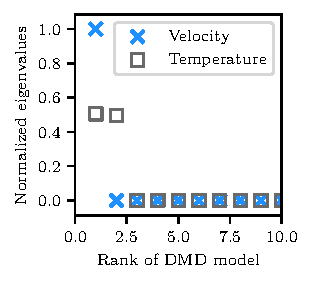
\includegraphics[width=\textwidth]{DMD_eigenspectrum}
    
    {\small
      Eigenspectrum of \( \bm{C}_{\bm{yx}} \bm{C}_{\bm{xx}}^{-1} \bm{C}_{\bm{xy}} \).
    }
  \end{minipage}
  
  \vspace{1cm}
\end{frame}

\begin{frame}[t, c]{Dynamic Mode Decomposition}{In practice}
  \begin{minipage}{.32\textwidth}
    \centering
    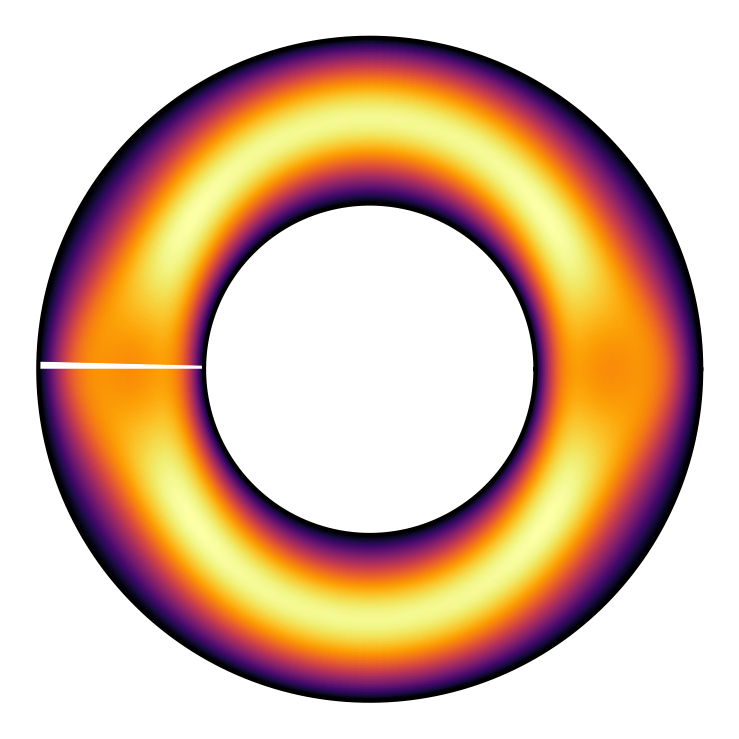
\includegraphics[width=\textwidth]{velocity_dmd_mode} \\
    
    {\small
      Leading DMD mode for the velocity.
    }
  \end{minipage}%
  \hfill
  \begin{minipage}{.32\textwidth}
    \centering
    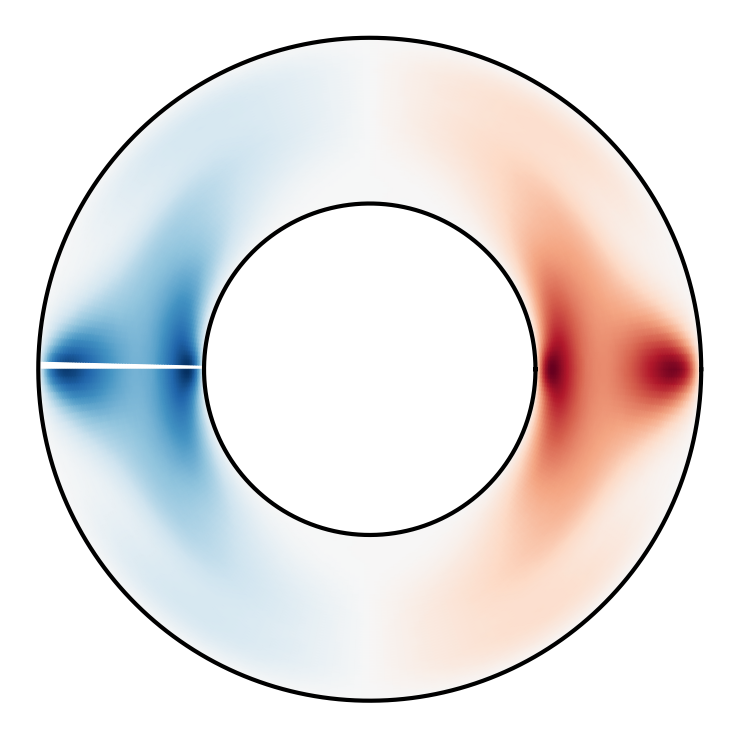
\includegraphics[width=\textwidth]{temperature_dmd_mode}
    
    {\small
      First DMD mode for the temperature.
    }
  \end{minipage}%
  \hfill
  \begin{minipage}{.32\textwidth}
    \centering
    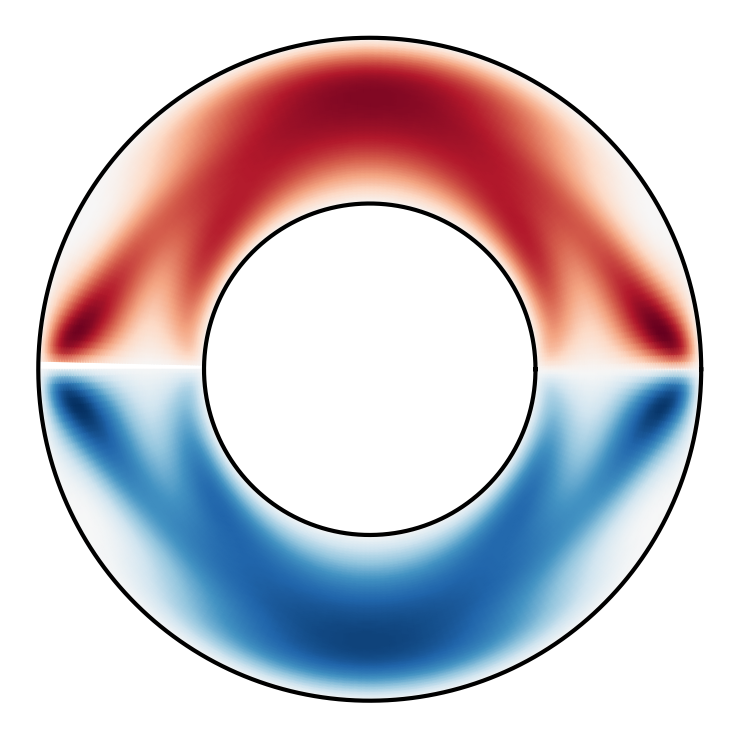
\includegraphics[width=\textwidth]{temperature_dmd_mode_bis}
    
    {
      \small
      Second DMD mode for the temperature.
    }
  \end{minipage}
  
  \vspace{1cm}
\end{frame}

\begin{frame}[t, c]{Dynamic Mode Decomposition}{In practice}
  \centering
  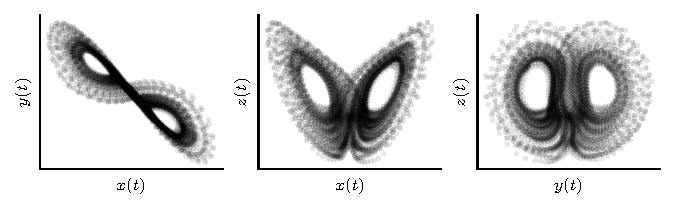
\includegraphics[width=.9\textwidth]{separate_low_dimensional_representation}
  
  \vspace{1cm}
\end{frame}
